\documentclass{bioinfo}
\copyrightyear{2011}
\pubyear{2011}

\begin{document}
\firstpage{1}

\title[a5]{A User-friendly Pipeline for de Novo Assembly of Microbial Genomes}
\author[Tritt \textit{et~al}]{Andrew Tritt\,$^{1}$ Jonathan A. Eisen\,$^{1,2,3}$ Marc T. Facciotti\,$^{1,4}$ and Aaron E. Darling,$^{1}$\footnote{to whom correspondence should be addressed}}
\address{$^{1}$Genome Center, $^{2}$ Dept. of Evolution and Ecology, $^{3}$ Medical Microbiology and Immunology, 
$^{4}$ Biomedical Engineering, University of California-Davis, Davis, CA 95616.}

\history{Received on XXXXX; revised on XXXXX; accepted on XXXXX}

\editor{Associate Editor: XXXXXXX}

\maketitle

\begin{abstract}
Remarkable advances in DNA sequencing technology have created a need for \textit{de novo} genome assembly methods
tailored to work with the new sequencing data types. Many such methods have been published in recent years, but assembling
raw sequence data to obtain a draft genome has remained a complex, multi-step process, 
involving several stages of sequence data cleaning, error correction, assembly, and quality control. 
Successful application of these steps usually requires intimate knowledge of a diverse set of algorithms and software. 
We present an assembly pipeline called A5 that simplifies the entire genome assembly process by automating these stages, by
integrating several previously published algorithms with new algorithms for quality control and automated assembly parameter selection.
We demonstrate that A5 can produce assemblies of quality comparable to a leading assembly algorithm, SOAPdenovo, without
any prior knowledge of the particular genome being assembled and without the extensive parameter tuning required
by the other assembly algorithm. The A5 pipeline can also assemble Illumina sequence data from libraries constructed by the Nextera
(transposon-catalyzed) protocol, which have markedly different characteristics to mechanically sheared libraries.
Finally, A5 has modest compute requirements, and can assemble a typical bacterial genome on current desktop or laptop computer hardware.

\section{Summary:}
\section{Availability:}
GPL source code, precompiled binaries for 64-bit Linux and Mac OS X, and a usage tutorial is available from \href{http://ngopt.googlecode.com}{http://ngopt.googlecode.com}

\section{Contact:} \href{mailto:andrew.j.tritt@gmail.com}{andrew.j.tritt@gmail.com}, \href{mailto:aarondarling@ucdavis.edu}{aarondarling@ucdavis.edu}
\end{abstract}

\section{Introduction}
High throughput DNA sequencing continues to revolutionize our understanding of biological systems. In particular,
the \textit{de novo} sequencing and assembly of genomes and metagenomes has yielded basic scientific insight into 
the relationship between genotype and phenotype,
in addition to biotechnological advances in enzyme discovery, bioprospecting, medicine, and agriculture.  
Although many high throughput sequencing instruments have been developed, such as the ABI SOLiD, Helicos Heliscope, IonTorrent PGM, Roche 454, and 
Pacific Biosciences RS1, we focus on data generated by the Illumina instrument in this work because it is the most prevalent data type at the moment. 
Current Illumina instruments such as the HiSeq 2000 and MiSeq generate paired nucleotide sequence reads of length up to150nt per read from fragments  
as long as 600nt. Currently one run of a HiSeq 2000 instrument generates up to 600Gbp of sequence data.  Despite the widespread use of Illumina  
sequencing, \emph{de novo} genome assembly from Illumina data continues to pose a challenging problem.



A tremendous number of software tools have been developed to assist with genome assembly from Illumina data.
These include tools for base calling of the images from the sequencer~\citep{BayesCall,Kircher2009},
error correction of the sequence reads~\citep{Kelley2010,Kao2011}, removal of adapter sequence contamination~\citep{Lassmann2009},
contig assembly~\citep{Warren2007,Chaisson2008}, and scaffolding~\citep{Koren2011,Boetzer2011,Dayarian2010}.
This list is not complete, but rather meant to illustrate some of the many tools for Illumina sequence analysis.
As part of a project to sequence and assemble \textit{de novo} the genomes of 64 halophilic archaea, we have
evaluated many of these software tools and constructed a new genome assembly pipeline that incorporates
methods for data cleaning, error correction, contig assembly, and scaffolding together with a new algorithm
for assembly quality control. 

The new assembly quality control algorithm uses paired-end read information
to detect and fix misassembled contigs and scaffolds. The first stage involves mapping reads back to assembled contigs.
The second stage involves detecting statistically significant clusters of read pairs that conflict with the
assembled contigs. Having identified putative regions of misassembly, the algorithm then determines the 
region of misassembly as precisely as possible and removes that region from the assembly, breaking the contigs
or scaffolds at that point. The quality control algorithm is implemented in a software module that can also be used 
independently of the assembly pipeline.

The new assembly pipeline, called A5, can operate directly on FastQ format data generated by an Illumina sequencing run
without any prior processing. The pipeline also contains methods to infer many of the assembly parameters directly
from the data, and in cases where that was not practical, default values have been chosen by tuning their values on 
assemblies of \textit{Haloferax mediterranei} and \textit{Haloferax volcanii}, for which reference genomes were available.

We present a comparison of A5 to SOAPdenovo on two datasets. The first dataset
is a halophilic archaeon for which a high quality reference genome is available. For this dataset we are able to use
reference-based assembly metrics to evaluate assembly quality~\citep{Darling2011}. We also evaluate assembly quality on an 
\textit{E. coli} isolate sequenced using transposon-catalyzed library preparation methods (Epicentre Nextera). 
No high quality reference genome exists for the \textit{E. coli} isolate, so we report basic descriptive statistics for assemblies
generated by each method.  

\begin{methods}
\section{Methods}

\subsection{A5 pipeline}

The A5 (\textbf{A}ndrew \textbf{A}nd \textbf{A}arons \textbf{A}wesome \textbf{A}ssembly) pipeline consists of five 
stages: 1) read cleaning, 2) contigging, 3) scaffolding, 4) misassembly checking, and 5) rescaffolding. 
Figure~\ref{fig:01} provides an overview of these stages. 

\subsubsection{Stage 1}
For the first stage A5 uses two previously published programs. First, 
ambiguous and low quality portions of reads are removed from the dataset. Then sequencing errors are corrected in the reads. Both of these 
steps use tools from from the SGA software package~\citep{Simpson2010}.  Although many read error correction packages have been published,
we found the implementation in SGA to have reasonable compute time and memory requirements compared to others while also providing 
good accuracy.  Next, the pipeline applies Tagdust~\citep{Lassmann2009} to remove any 
sequencing adapter contamination that may be present in the data. The default set of adapter sequences used for screening
include the standard Illumina TruSeq adapters and those used in Epicentre Nextera (transposon-catalyzed) library preparation protocols~\citep{Adey2010}. 
User-specified adapter sequences can be screened by adding them to a FastA file. 

\subsubsection{Stage 2}
Using the newly cleaned reads derived from stage 1, stage 2 of the pipeline builds contigs
with the the assembler IDBA~\citep{Peng2010}. We selected IDBA due 
to its ability to produce long contigs in the presence of inconsistent depth of sequence coverage more robustly than other methods (data not shown).
Like many current assembly algorithms, IDBA uses a \emph{de Bruijn} graph-based algorithm to assemble contigs. A \emph{de Bruijn} graph is a directed graph 
that represents overlap between all $k$-mers found in a nucleotide dataset. For a more complete description and comparison to other assembly 
approaches please see~\citet{Pop2009}. Many \emph{de Bruijn}-based assemblers require the user to specify a single $k$-mer length, and the optimal 
choice of $k$ depends intimately on characteristics of the genome being assembled.  Moreover it is possible that for a particular dataset with given 
read lengths and error profiles, different regions of the same genome may be optimally reconstructed by different values of $k$. In contrast, IDBA
simply requires a minimum and maximum value of $k$ to use when processing the \emph{de Bruijn} graph into contigs. This simplifies parameter choice. 
One final factor entering into the choice of IDBA was its 
ability to generate highly contiguous sequence even with unpaired sequence reads. Although assemblers using paired-end read information during 
contigging can often produce exceptional results~\citep{Gnerre2011, SASSY}, we did not want to impose the requirement of paired reads (or multiple
libraries with different insert sizes) upon users of the pipeline. This keeps applicability of A5 as broad as possible.

\subsubsection{Stage 3}
In stage 3 of A5, contigs are scaffolded and extended using the software SSPACE~\citep{Boetzer2011}. 

\subsubsection{Stage 4}
In stage 4 of A5, crude 
scaffolds are subjected to a quality control check for misassemblies. 
An undesirable side-effect of using a contigging algorithm that is unaware of read pairing information is that misassemblies can occur in contigs 
that could have been avoided if the longer-range linkage information present in read pairs (or long reads) had been used.  As described in Results 
below, we observe occasional misassemblies in the contigs generated by IDBA. Although the version of IDBA currently incorporated into A5 (v0.20) has
an option to use pairing information, it has little effect on the assembly (data not shown). 
Cleaned reads are mapped back to crude scaffolds using the read mapping software,
BWA~\citep{bwa}. Custom code (described in detail below in section \ref{sec:qc}) is then used to extract all read pairs that are discordant with the 
crude scaffold assembly and two-dimensional spatial clustering~\citep{DBSCAN} is used to identify clusters of discordant read pairs that are 
suggestive of a misassembly. The A5 pipeline then breaks the crude scaffolds at the estimated position of the misassembly.

\subsubsection{Stage 5}
Finally, in stage 5 the broken-up scaffolds are rescaffolded using SSPACE~\citep{Boetzer2011}.
\end{methods}


\begin{figure}[t]
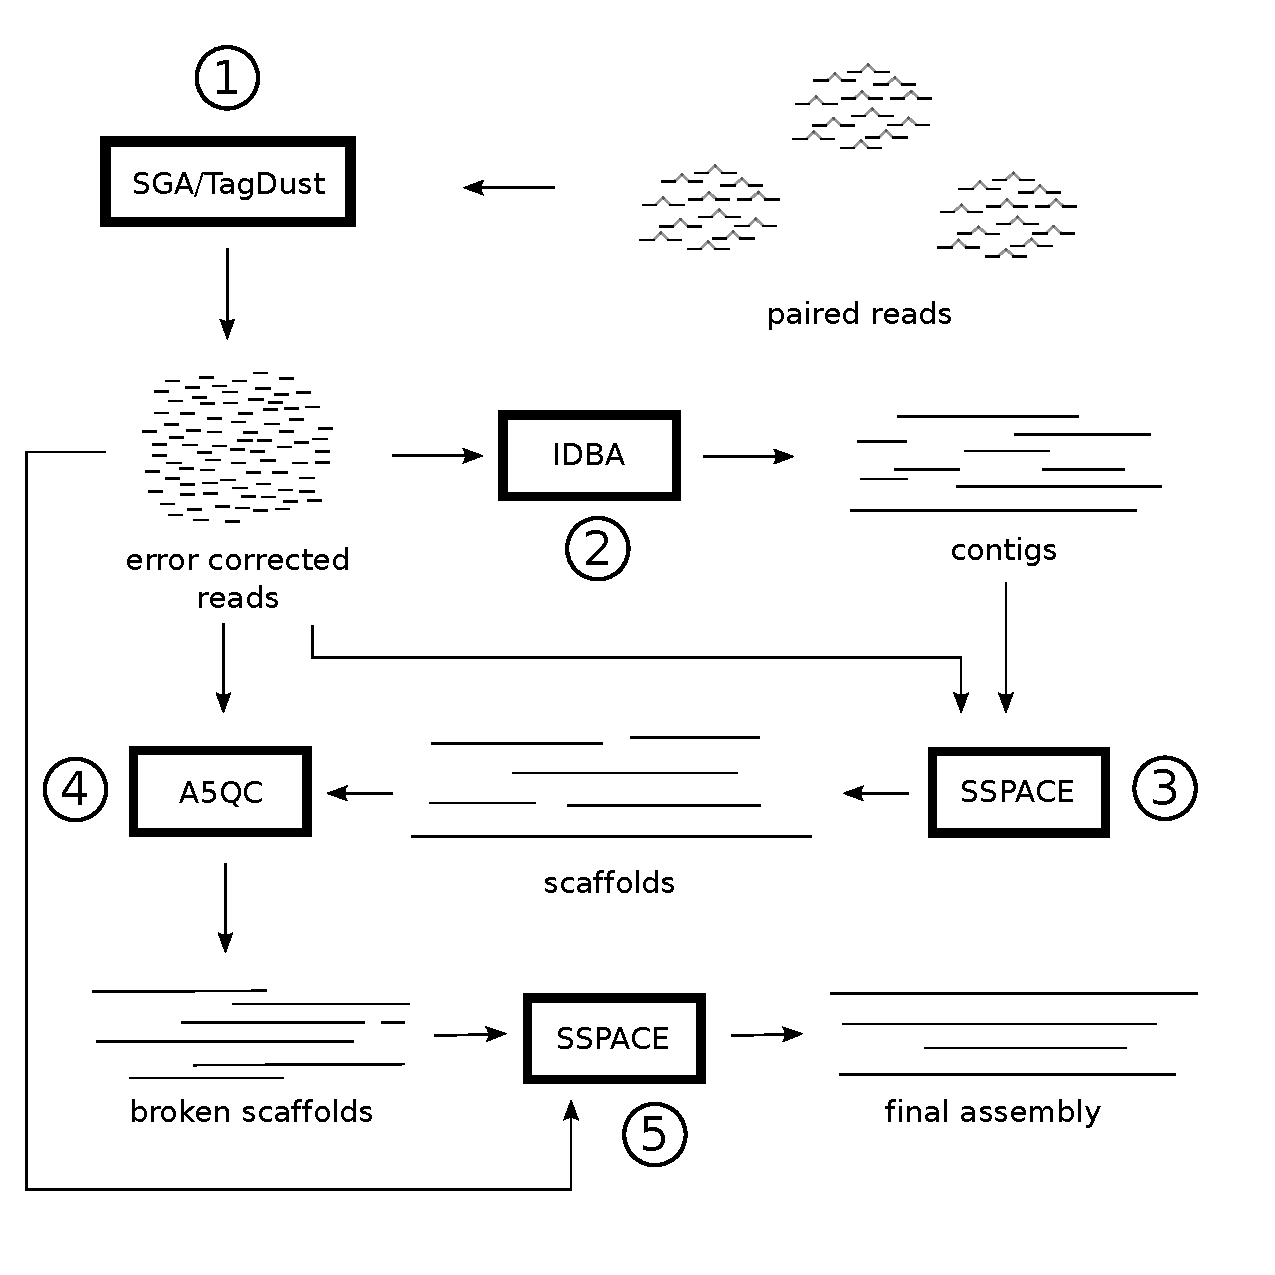
\includegraphics[width=3.5in]{a5pipeline-diagram.pdf}
\vspace{-1cm}
\caption{Overview of the stages in A5. The first stage of the pipeline is to clean reads, removing any contaminant
reads and correcting base-call errors. Then the pipeline assembles contigs with IDBA using these error corrected reads. These
contigs are then scaffolded using the original read set. Scaffolds are then checked for misassemblies, and broken at regions
containing misassemblies. Finally, the broken scaffolds are rescaffolded using the original read set.}\label{fig:01}
\end{figure}

\subsection{Automated parameter selection}

Most currently available assembly programs have a wide variety of parameters which must
be specified by the user, and some of these can have a profound impact on the quality of the 
resulting assembly. The software employed within A5 is no exception. 
Often these parameters require dataset-specific tuning.  A common approach
employed by the hapless bioinformatician involves repeatedly
executing the assembly software and evaluating the results until a perceived 
optimum has been achieved (or a pressing deadline looms). Scripts for automating this iterative tuning procedure have 
been developed~\citep{VelveltOpt}, however, it is not always feasible, depending on available compute resources and the size 
of the dataset. The A5 pipeline avoids the problem for users by calculating reasonable
parameters for each stage of the pipeline using values derived from the data itself. In some
cases, default parameters have been set to data-independent values. Supplementary Table~\ref{Tab:03} 
summarizes the many parameters in the pipeline.

\subsection{Automated misassembly quality control}\label{sec:qc}

After crude scaffolds have been built, A5 performs an automated quality control step.

As exemplified in Figure 2, reads are first mapped to scaffolds, and then read pairs are spatially clustered on the
points where they map. After mapping, read pairs that support the current assembly architecture, which we 
refer to as \emph{proper connections}, must be removed before spatial clustering. Without their removal, \emph{proper connections}
among read pairs would form large spatial clusters. Including these data in the clustering input would not only waste considerable 
computational resources but may also obscure or subsume clusters caused by local misassemblies in scaffolds. 


Proper connection scan be identified using the DNA fragment length (insert size) distribution of the library. However, two common features of
Illumina datasets can skew the mean and inflate the variance estimates of the insert size distribution. The first of these features is referred 
to as a \emph{shadow} library. Briefly, a shadow library is a population of small-insert ($<$600nt) paired end reads that are a product of 
imperfect construction of large-insert mate-pair libraries using the standard Illumina protocol. The Illumina mate-pair protocol involves 
circularization of fragments, further subfragmentation of the circular molecules, and purification of the linear subfragments containing the circularization junction. 
The purification of subfragments containing circularization junctions (from which the large-insert mate-pair reads derive) often fails to remove all 
DNA fragments lacking a circularization junction, those fragments yield the small insert read pairs termed a \emph{shadow} library. The second 
feature that can interfere with insert size distribution calculations is inherent noise in the dataset. Such noise can be caused by chimeric 
fragments and ambiguous read mapping due to repetitive regions or highly erroneous reads. 


\subsubsection{Accurate estimates of insert size distributions}

To avoid including noise in mean and variance estimates from shadow libraries and other error sources, 
we perform a round of Expectation-Maximization (EM) clustering of insert sizes before calculating sample statistics~\citep{GuptaChen2010}. 
Choice of the number of clusters $K$ in
the EM-clustering algorithm is derived from a preliminary estimation of the library insert size using the method implemented in
BWA~\citep{bwa}. Libraries with a preliminary
insert size estimate greater than 1000 bp are assumed to have been constructed using a mate-pair protocol, and therefore
may contain a paired-end short insert shadow library in addition to the large insert mate-pair library. To separate the short insert library
from the large insert library, $K$ is set to 3: one cluster for improper connections, one cluster for the short insert
shadow library, and one for the desired large insert library. If the preliminary insert size estimation is less than 1000 bp, the library
is assumed to have been constructed using a paired-end protocol, and $K$ is set to 2: one for improper connections
and one for the short-insert library. Clusters returned from EM-clustering are identified as containing improper connections if 
they have high variance, defined as $s > \mu$, and proper connections if they have low variance ($s \le \mu$), where $\mu$ is the mean insert of pairs within
the cluster, and $s$ is the standard deviation. In practice, the $(K-1)$th lowest-variance clusters are identified as proper connections.
Each low-variance cluster is then used to remove mapped read pairs 
having inserts in the range $(\mu-ns,\mu+ns)$, where $n = \min(\lfloor\frac{\mu}{s}\rfloor, 6)$.  The remaining read
pairs represent improper connections and may contain clusters suggestive of misassembly.


\begin{figure}[t]
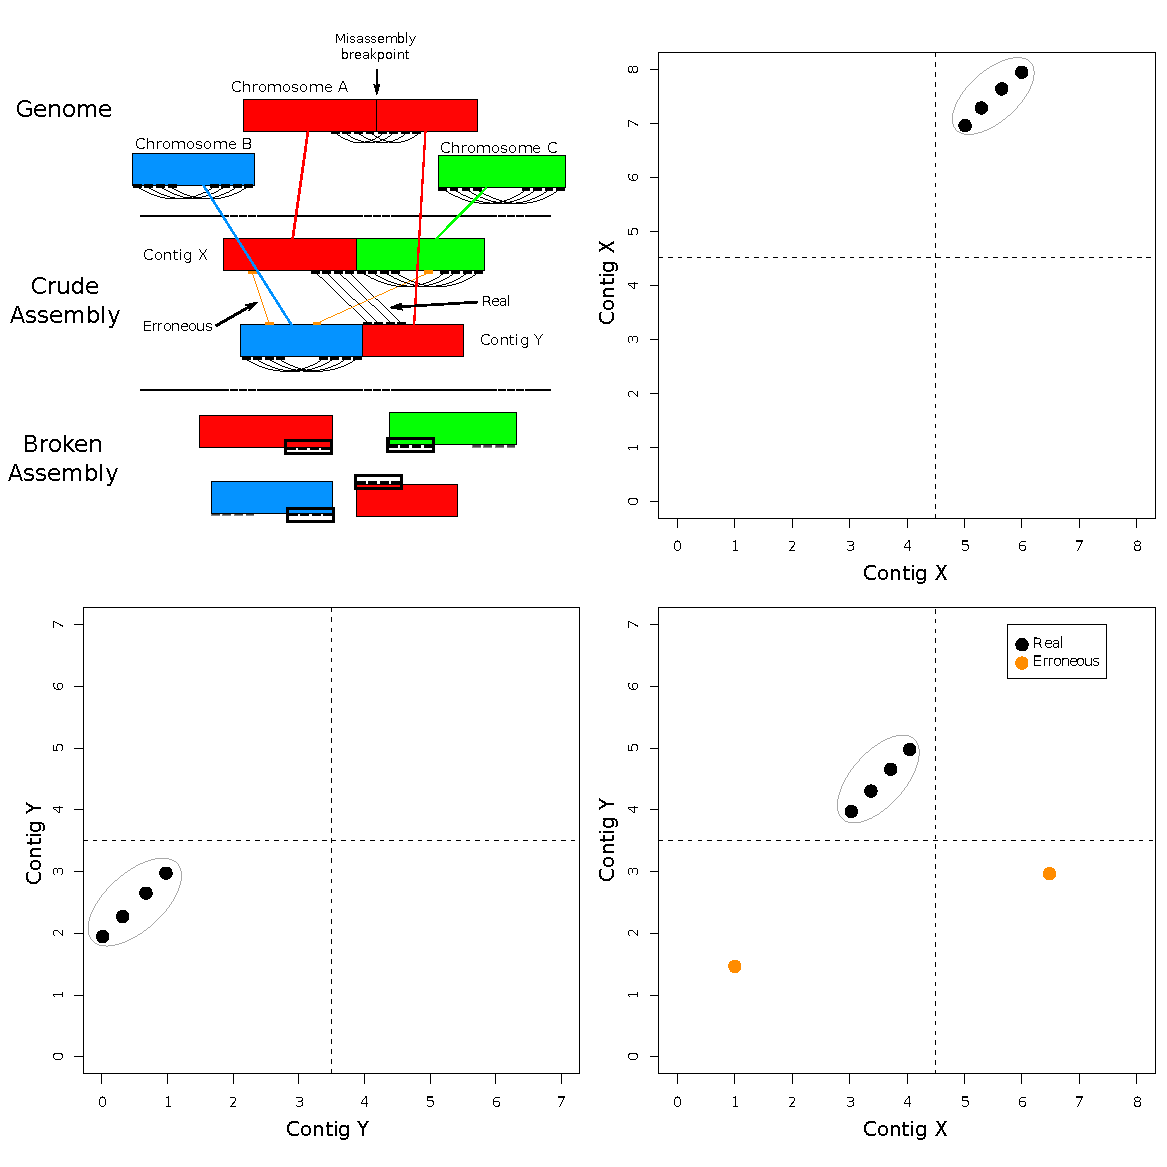
\includegraphics[width=3.5in]{a5qc.pdf}
\vspace{-1cm}
\caption{\textbf{Upper Left:}  A hypothetical whole genome alignment of an assembly containing misassemblies relative to the true genome,
consisting of three circular chromosomes, and the 
resulting broken assembly. Red, green, and blue lines connect aligned regions. Black connecting lines represent real paired read 
connections between contigs and orange connecting lines represent erroneous connections. Black boxes in the broken assembly highlight
blocks identified by the DBSCAN algorithm. \textbf{Upper Right and Bottom Row:} Plots of connected points between contigs. Black and orange dots 
correspond to black and orange connections lines from left figure, respectively. Dotted lines correspond
to misassembly breakpoints. Gray circles highlight the set of points that are clustered by DBSCAN. }\label{fig:02}
\end{figure}

After proper connections have been removed, misassemblies are identified by locating clusters of many read pairs mapped within
a scaffold or between two scaffolds. We treat the mapped read pairs as \emph{points} in
two-dimensional spaces defined by each possible scaffold pair and self-pair. When the outer boundaries of a cluster of points
is projected back onto the one dimensional sequence(s), we call the resulting intervals \emph{blocks}.
These blocks define regions of misassembly.

To identify blocks, we use the spatial clustering algorithm DBSCAN 
to cluster points in each of these 2-dimensional spaces~\citep{DBSCAN}. The two key parameters of DBSCAN are $\varepsilon$, the maximum allowed
distance between two points in a cluster and $MinPts$, the minimum number of points allowed in a cluster. The first parameter is used to locate 
the neighboring points of each point, where a point $b$ is considered a neighbor of point $a$ if $|a_x - b_x| < \varepsilon 
~~\mbox{and}~~ |a_y - b_y| < \varepsilon$. We set $\varepsilon$ by modelling read mapping positions as a Bernoulli process. 
The probability of success $p$ in the Bernoulli process is set by calculating a minimum read mapping frequency across the genome assembly.
This is done by partitioning the assembly into windows of length $L$, where $L = \max(1000,\mu)$ for a library with mean insert $\mu$. 
Let $w_i$ be the $i$th window and $n_i$ be the number of reads that map to $w_i$. We then set $p$ according to the following equation
\begin{equation}
	p = \dfrac{\min_{i}(n_i)}{L}
\end{equation}
The rationale for using the portion of the crude scaffold assembly with the fewest mapped reads is that in practice, sequencing
coverage is often highly variable, with some regions receiving excessive coverage and others receiving little. This variation
in coverage can be caused by systematic biases in the library construction and sequencing procedures, including fragmentation bias,
PCR bias, and uneven representation of genomic DNA after DNA extraction. By estimating this parameter on a region of low
coverage, we ensure sensitivity to detect misassemblies in low-coverage regions.

Assuming the positions of mapped reads  
follow a Bernoulli process, the distance between two independent reads in a sequence follows a geometric distribution with parameter $p$.
We derive a maximum allowable distance, $d(p)$, between two points (mapped reads) in one sequence by selecting the
$1-\alpha$ quantile of a geometric distribution with parameter $p$. This is done by setting the cumulative distribution function, $1 - (1-p)^k$, equal to $1-\alpha$ and solving for $k$:
\begin{eqnarray}
	1 - (1-p)^{k} = 1-\alpha \nonumber \\
	(1-p)^{k} = \alpha  \nonumber \\ 
	k*\ln(1-p) = \ln(\alpha)  \nonumber \\
	k = \dfrac{\ln(\alpha)}{\ln(1-p)} = d(p)
\end{eqnarray} 
for some $\alpha < 1$. In practice we set $\alpha = 0.001$, to select the 99.9$^{th}$ quantile. Furthermore, we assume overlapping reads belong to
the same block, and set $\varepsilon = \max(d(p),l_r)$ where $l_r$ is the read length.
The second parameter of the DBSCAN algorithm, $MinPts$, is set to be the expected number of points in the minimum allowed block length in a region
of minimal coverage. Assuming a block will consist of
3 points at minimum and allowing a maximum distance between consecutive points to be $\varepsilon$, we allow the minimum block length to be 
$\ell{_{min}} = \lfloor2\varepsilon\rfloor$. We then calculate the expected number of points in a window of length $\ell{_{min}}$ given that the probability of
a read mapping to a single position is $p$, setting $MinPts = \lfloor{p\ell{_{min}}}\rfloor$. 

Finally, regions of length $\le 2\mu$ within individual scaffolds that are flanked by two blocks are identified as containing
misassemblies and are removed from the assembly, breaking the scaffold into two subscaffolds. The removed region contains the 
misassembly breakpoint, but the exact position of the misassembly may not be well-defined in many cases, either due to lack of
coverage by reads spanning that position or due to errors in the assembled sequence.



\section{Results}

\begin{table*}[!t] 
\processtable{ Reference-based assembly metrics on ten assemblies of \textit{Haloferax volcanii} DS2 
(\textbf{Volc}) dataset. ``scaf'' indicates an assembly that has been scaffolded, while ``ctg'' indicates no scaffolding. 
Labels ``-CDS'', ``-N50'', and ``-LCB'' indicate SOAPdenovo assemblies run with parameters combinations that minimized broken coding 
sequences, maximized scaffold N50, and minimized LCB (Locally Collinear Block) count, respectively. For A5, assembly ``scaf-QC'' has been 
broken using the A5QC algorithm and rescaffolded using SSPACE. The DCJ Distance is the Double-Cut-and-Join distance~\citep{Bergeron2006},
a measure of the minimum number of rearrangement operations required to transform one genome assembly into another.
\label{Tab:01}}
{\begin{tabular}{l|cccccc|ccc}\toprule
&\multicolumn{6}{c|}{SOAPdenovo} & \multicolumn{3}{c}{A5} \\
Assembly           & ctg-CDS & scaf-CDS & ctg-N50 & scaf-N50 & ctg-LCB & scaf-LCB & ctg    & scaf     & scaf-QC   \\\midrule
Sequence count     & 7686    & 211      & 10258   & 212      & 19508   & 226      & 853    & 106      & 95      \\
N50                & 5111    & 125642   & 4775    & 125739   & 2832    & 107081   & 8170   & 101041   & 110196  \\
Miscalled bases    & 379     & 573      & 270     & 395      & 409     & 377      & 120    & 315      & 247     \\
Uncalled bases     & 0       & 92290    & 0       & 11430    & 0       & 13304    & 0      & 6436     & 6727    \\
Extra bases        & 269960  & 18582    & 27069   & 14295    & 32797   & 19732    & 14096  & 17903    & 18496   \\
Missing bases      & 149253  & 151966   & 148291  & 142017   & 160773  & 156254   & 128909 & 107421   & 106626  \\
Extra sequences    & 6129    & 75       & 8604    & 76       & 17194   & 95       & 33     & 5        & 5       \\
Missing replicons  & 0       & 0        & 0       & 0        & 1       & 1        & 0      & 0        & 0       \\
DCJ Distance       & 1559    & 143      & 1656    & 140      & 2317    & 134      & 839    & 123      & 100     \\
LCB Count          & 15      & 22       & 9       & 14       & 7       & 10       & 45     & 55       & 28      \\
Broken CDS         & 434     & 434      & 454     & 454      & 634     & 634      & 276    & 214      & 212     \\
\botrule \\
\end{tabular}}{}
\end{table*}

% TnSOAPdenovo__MaxN50 : K = 27, d = 2

\begin{table*}[!t]
\processtable{ Non-reference based metrics on six assemblies of \emph{Escherichia coli} CC118 (\textbf{Tn}) dataset. Data
for SOAPdenovo were calculated from the assembly run with parameters that maximized scaffold N50. 
``scaf'' indicates an assembly that has been scaffolded, while ``ctg'' indicates no scaffolding. For A5, assembly ``scaf-QC'' has been 
broken using the A5QC algorithm and rescaffolded using SSPACE. 
\label{Tab:02}}
{\begin{tabular}{l|cc|ccc}\toprule
& \multicolumn{2}{c|}{SOAPdenovo} & \multicolumn{3}{c}{A5} \\
Assembly        & ctg     & scaf    & ctg     & scaf    & scaf-QC \\\midrule
Sequence count  & 4348    & 197     & 323     & 111     & 87      \\
N50             & 12825   & 83067   & 27846   & 72166   & 82719   \\
Mean seq len    & 1056    & 22647   & 13800   & 40207   & 51300   \\
Max seq len     & 48725   & 200327  & 113049  & 330689  & 330689  \\
Total bases     & 4590705 & 4461465 & 4457409 & 4462953 & 4463084 \\
Uncalled bases  & 0       & 26290   & 0       & 220     & 290     \\
\botrule \\
\end{tabular}}{}
\end{table*}

We evaluated the performance of A5 on two real Illumina data sets and compared the results to
those obtained when running SOAPdenovo v1.05~\citep{Li2010} on the same datasets. The first data set (called \textbf{Volc}) is a paired-end short insert library constructed from \emph{Haloferax volcanii} DS2 genomic DNA 
using sonication followed by end-repair, A-tailing, and adapter ligation, and was sequenced on an Illumina GAIIx instrument.
Sequencing yielded 6,844,701 read pairs, with each read being 78nt in length. These data have been deposited at the NCBI Short Read Archive, accession SRX105348 (data can be downloaded
from http://edhar.genomecenter.ucdavis.edu/~andrew/ngopt\_pipeline/ms/). 
The second data set, called \textbf{Tn} and previously published by \citet{Adey2010}, is a paired-end library constructed from \emph{Escherichia coli} CC118 genomic DNA
using transposon-catalyzed adapter ligation (Nextera) and was sequenced on an Illumina HiSeq2000 instrument using TruSeq 2 chemistry. 
Reads from this dataset were obtained from the NCBI Short Read Archive, accession SRX030179.

We executed A5 and SOAPdenovo for each data set. Table 1 reports the assembly performance for \textbf{Volc} assemblies.
Table 2 reports the assembly performance for \textbf{Tn} assemblies. \textbf{Volc} assemblies were scored using Mauve Assembly 
Metrics~\citep{Darling2011}, which quantifies differences between the reference and assembly using whole genome alignment. We note that
aligner error may result in additional errors between the assembly. Although high quality reference assemblies exist for other \textit{E. coli} 
isolates, none are available for strain CC118. We can not use another \textit{E. coli} as a reference due to the great deal of genomic divergence
among \textit{E. coli} isolates~\citep{Perna2001}.
 Contigs from A5 were broken using the A5QC algorithm. \textbf{Volc} contigs were broken up into XXX contigs (N50 = XXX) and \textbf{Tn} contigs were broken up into YYY contigs (N50 = YYY). 

We initially ran SOAPdenovo with default parameters; however, the resulting assemblies were of extremely poor quality. For \textbf{Volc} there were
280985 contigs (N50 = 76) and 14433 scaffolds (N50 = 209), and for \textbf{Tn}, there were 1572720 contigs (N50 = 76) and 8144 scaffolds (N50 = 121). 
Rather than reporting poor results for SOAPdenovo, we endeavored to manually optimize its assembly parameters so that we can compare the A5 assembly
to the best possible SOAPdenovo results. 
To do so, we ran SOAPdenovo with different combinations of values for the parameters $K$ and $d$, where $K$ is the $k$-mer size for SOAPdenovo and $d$
is the threshold for the minimum number of times a $k$-mer must be observed in the data to be considered valid.
For both datasets, we selected combinations that maximized scaffold N50. In addition, for the \textbf{Volc} dataset we also present assembly scoring
results for the parameter combination that minimized LCB (locally colinear block) count between the assembly and the reference, as well the combination that minimized the
number of broken coding sequences. The parameter combination that maxmized scaffold N50 for \textbf{Volc} also minimized the sum
of missing and extra bases relative to the reference. The parameter space queried was $S_K \bigoplus S_d$,
where $S_K = \{23,25,27,29,31\}$ is the set of values over which $K$ was varied, and $S_d = \{1,2,...,9,10\}$ is the set of values over which $d$
was varied. 
Using this process, the optimal parameters were found to be
\begin{itemize}
\item \textbf{Volc} (-N50): $K = 27$, $d = 2$.
\item \textbf{Volc} (-LCB): $K = 27$, $d = 1$.
\item \textbf{Volc} (-CDS): $K = 29$, $d = 2$.
\item \textbf{Tn}: $K = 27$, $d = 2$
\end{itemize}

A5 assemblies were generated using source code from revision 625 of A5.

\begin{figure}[t]
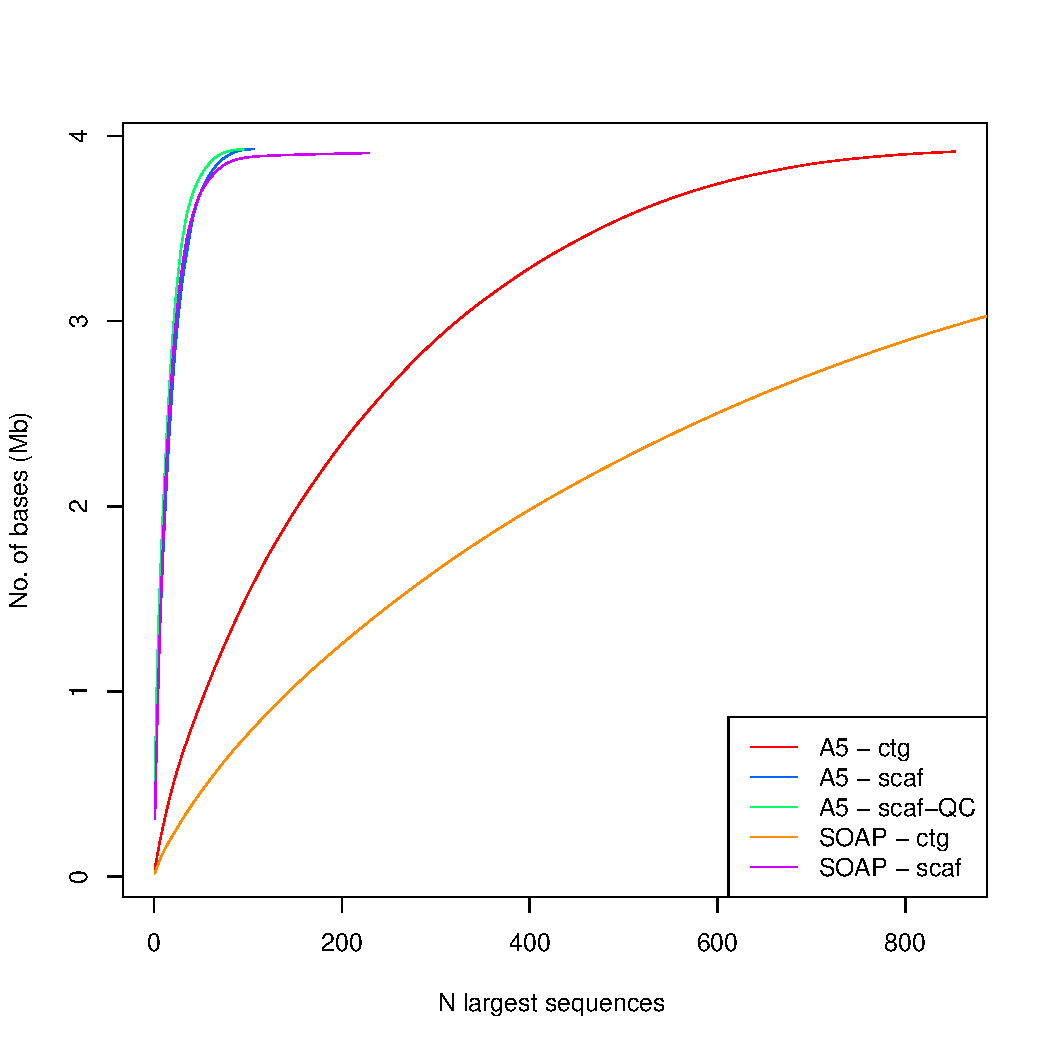
\includegraphics[width=3.5in]{volc_accum_plot.pdf}
\vspace{-1cm}
\caption{Sequence length accumulation curve for six assemblies of the model archaeon \textit{Haloferax volcanii} DS2. Curves represent the number of bases 
in an assembly as a function of the $N$ largest sequences. Assemblies generated from SOAPdenovo and A5 are labelled with ``SOAP'' and ``A5'', 
respectively. ``scaf'' indicates an assembly that has been scaffolded, while ``ctg'' indicates 
no scaffolding. For A5, assembly ``scaf-QC'' has been broken using the A5QC algorithm and rescaffolded using SSPACE.
A perfect assembly would have exactly the number of sequences as the organism has replicons (5 in this case), and the curve would be
in the extreme upper left corner.}\label{fig:03}
\end{figure}

\section{Discussion}

When little is known about the data being assembled, A5 produces higher quality assemblies 
than SOAPdenovo. To obtain the SOAPdenovo results we conducted a parameter sweep 
over 50 combinations of $k$-mer length ($K$) and the minimum $k$-mer frequency ($d$), while A5 required
only a single run of the pipeline.
SOAPdenovo outperforms A5 in scaffold count and N50 on the \textit{Haloferax volcanii} DS2 dataset, but on the \textit{E. coli} dataset 
(for which no high quality reference assembly is available) 
A5 produces a better assembly when measured by scaffold count, mean scaffold size, and max scaffold size.
One possible reason that A5 may produce better results on the transposon catalyzed library is that the insert size using
that library preparation protocol often does not fit a normal distribution.  Instead the insert size 
distribution depends greatly on the relative concentrations of transposase and target DNA and can range from a truncated uniform
to roughly lognormal depending on the enzyme concentration and what size selection steps are taken during library preparation.
Most scaffolding programs to-date model the insert sizes for paired-end reads using a normal distribution with a particular
mean and standard deviation. A5 also uses this model, but has been configured to be permissive of scaffolding
using libraries with broadly distributed insert sizes.  A second possible explanation for A5's improved performance on transposon-catalyzed 
libraries may be that method is more robust to low coverage regions.  Illumina libraries constructed by in-vitro 
transposition with Tn5 transposase have considerable target site preference (data not shown), leading to highly nonuniform coverage around a genome.

In all cases where reference data was available A5 produced fewer miscalled bases. This is to
be expected, as A5 first performs error correction on reads before assembling them into contigs. A5 also produced assemblies
with fewer broken CDS. This is critically important for downstream analysis of gene function, regulation, and metabolism.


The strategy used for detection of misassmblies demonstrates the utility of paired-end data for improving draft genome assemblies.
In addition to identifying misassemblies after scaffolding, paired-reads may also be used to identify repetitive regions.   
Although we use paired short reads, the methodology is not limited to this type of data. Long reads with split mapping positions 
could in theory be used in the same manner as the paired short read data.

A limitation to misassembly detection is the underlying assumptions about the structure of misassemblies. The first assumption we make
is that the only feature of the misassembly is a false adjacency between two bases.
In many cases, however, a misassembly consists of more than a single false adjacency and includes extra inserted sequence.  One approach to
overcome this would be to employ a model that characterizes the insertion of additional sequence. A related limiting assumption is 
that coverage within each of the two regions surrounding the missassembly is uniform. This assumption is frequently violated, as sequence coverage
is rarely uniform. We also assume that coverage is equal on both sides of the false adjacency. In cases where coverage is not equal between 
the two regions flanking a misassembly, as may be the case in metagenomes, a spatial clustering algorithm that allows for variable density
clusters, such as AMSTLSC~\citep{AMSTLSC}, would more accurately identify blocks. Finally, we assume that all replicons in the target genome
are circular. In genomes containing linear chromosomes, a misassembly combining a whole linear chromosome with another chromosome
at a non-telomeric region would result in a single block on one side of the misassembly. Identifying a misassembly in this case
would require additional information. When two chromosomes have been assembled together at their telomeres, no such blocks will be found, 
necessitating a different approach to identifying misassemblies.

In addition to theoretical limitations, A5 also also has practical computational limits. Large datasets, such as a full lane of data
generated on the Illumina HiSeq2000 platform, require resources beyond that typically available in a desktop or laptop computer. 
The major computational bottlenecks of A5 are the first two stages: read cleaning and contigging. Memory requirements for read error
correction grow with total data volume, requirements for contigging grow with data volume and total size/complexity of the assembled genome 
(since the \textit{de Bruijn} graph is more complex in these cases).
The DBSCAN algorithm has $O(n\log{n})$ time-complexity and $O(n)$ memory-complexity. One 
approach to reduce the memory complexity of DBSCAN would be to implement a grid-based density clustering algorithm that operates on cell densities 
rather than individual data points. Such algorithms exist~\citep{STING}; however, employing a grid may compromise the resolution at which 
a misassembly can be identified. Finally, when coverage is high, subsampling the dataset can lower the memory load without sacrificing
sensitivity.

Previous efforts have been made toward identification of misassemblies~\citep{Phillippy2008}. Implementations identify locations of putative 
misassemblies and require further manual inspection to remove these regions. The algorithm we developed for misassembly detection is conceptually 
similar to algorithms applied for segmental homology detection that operate by ``chaining'' homologous fragments into collinear blocks. Chaining 
algorithms such as FISH~\citep{Calabrese2003} and DAGChainer~\citep{Haas2004}, are not permissive for this task, as they depend on a 
collinear arrangement of points. Because fragment lengths vary in size, points of mapped read pairs rarely fit this model of collinearity. The algorithm is also related to structural variant detection 
algorithms ~\citep{BreakDancer,SVDetect}. Structural variant detection begins with mapping reads back to the reference and using read orientation 
information and mapping distance to identify anomalous pairs. In theory, some of these algorithms could also be employed to detect misassembly.  

\emph{de novo} genome assembly from Illumina data is an extremely active area of research, with many assembly algorithms published and many more continuing to be produced.
A thorough comparison of the performance of all these methods is a highly nontrivial undertaking and well outside the scope of the present  
work. Instead, we chose to compare A5 to a single other widely-used assembly method, namely SOAPdenovo. We selected SOAPdenovo for comparison
because it ranked among the best in two recent surveys of assembly algorithms~\citep{Earl2011,Salzberg2011}, because it is able to run on a single paired-end
library, and like A5 is relatively simple to download, install, and use. Although methods that require both small insert paired-end libraries
and large insert mate-pair libraries can produce very high quality results~\citep{Gnerre2011}, the time, cost and technical expertise required to construct large insert
libraries is significantly beyond that required for small insert libraries (especially using transposon-catalyzed library construction).
For this reason we feel there is a great need for methods to easily produce assemblies of the highest quality possible without large insert mate-pair data.
A5 can be considered a first attempt at such a method.

\section*{Acknowledgements}
This work was supported by National Science Foundation award ER 0949453. We thank Vadim Mozhayskiy for beta testing a
version of the A5 software.

\bibliographystyle{natbib}
\bibliography{a5pipeline-appnote}


% vSOAPdenovo__MaxN50      : K = 27, d = 2
% vSOAPdenovo__MinEMBases  : K = 27, d = 2
% vSOAPdenovo__MinBrCDS    : K = 29, d = 2
% vSOAPdenovo__MinLCB      : K = 27, d = 1

\section{Supplementary Material}
\subsection{Description of internal assembly pipeline parameters}

The A5 pipeline incorporates many algorithms, each of which require certain parameters to be set.
Table~\ref{Tab:03} lists all of the parameters used in A5, along with how the value
of that parameter is calculated. We now discuss the effect of each of these parameter settings in turn.  
The SGA Quality Trim parameter sets a PHRED Q-score cutoff~\citep{Ewing1998} used for read trimming with the algorithm
implemented in BWA~\citep{bwa}. The SGA Quality Filter parameter sets a maximum number of bases
with a PHRED Q-score of below 3 that are permitted in a read before the read is discarded entirely.
The SGA Min Read Length sets the minimum allowed read length after quality trimming, reads shorter
than that will be discarded.

The IDBA min $k$-mer sets the starting $k$-mer size for \emph{de Bruijn} graph construction, and the max $k$-mer sets
the largest $k$ that will be used during graph simplification.

The SSPACE Overhang MinOverlap sets the number of nucleotides that a read must overlap with an existing
contig to be used for contig extension during scaffold gap filling. The SSPACE ExtendCall MinBases sets the minimum
number of reads covering a base that are required to call the base during contig extension. The SSPACE minimum
links sets the minimum number of read pairs that must be connecting a pair of contigs in order for them to be considered
for scaffolding, the reads must map to the region of the contig expected based on the insert size distribution.
For three contigs A, B, and C, where read pairs link A,B and A,C, the SSPACE Min Link Ratio sets the 
maximum allowable ratio between the number of links connecting A,C and A,B. If the ratio is below the threshold,
A,B will be scaffolded, otherwise A will not be scaffolded. Here A,B and A,C have the highest and 2$^{nd}$ highest number
of links between A and any other contig.

The SSPACE Merge MinOverlap sets the minimum number of bases that two scaffolded contigs must overlap in order to be merged
into a single contig.  The SSPACE Insert Mean is the mean value of the insert size for a paired-end or mate-pair library. 
The SSPACE Insert StDev is the standard deviation.


\begin{table*}[!t]
\processtable{\textbf{Supplementary} Assembly parameters within the pipeline and how their values are chosen. 
$\varepsilon$ is the maximum inter-point distance used for spatial clustering and $MinPts$ is the minimum number of points
in a cluster.
\label{Tab:03}}
{\begin{tabular}{l|c|l}\toprule
Parameter                       & Stage & Default setting  \\\midrule
SGA Quality Trim (-q)           & 1     & hard coded to 10 \\
SGA Quality Filter (-f)         & 1     & hard coded to 20  \\
SGA Min Read Length (-m)        & 1     & hard coded to 30 \\
IDBA min $k$-mer                & 2     & 29, most $k$-mers of this size are unique in a microbial genome but larger values may be better for larger genomes \\
IDBA max $k$-mer                & 2     & maximum read length of trimmed reads \\
SSPACE Overhang MinOverlap (-m) & 3,5   & Max of 15 and floor of binary logarithm of genome size, plus 3.99  \\
SSPACE ExtendCall MinBases (-o) & 3,5   & hard coded to 1 \\
SSPACE Minimum Links (-k)       & 3,5   & base 1.4 logarithm of $E\_links$, minus 11.5, where $E\_links$ = $\dfrac{2c\mu}{l_r}$ and $c$ is coverage \\
SSPACE Min Link Ratio (-a)      & 3,5   & hard coded to 0.6,0.3  \\
SSPACE Merge MinOverlap (-n)    & 3,5   & floor of (binary logaritm of mean insert size, scaled by 1.24, plus 0.99) \\
SSPACE Insert Mean 	            & 3,5   & Calculated using EM-clustering \\
SSPACE Insert StDev             & 3,5   & Calculated using EM-clustering \\
DBSCAN $\varepsilon$            & 4     & Derived from coverage as described in main text \\
DBSCAN $MinPts$                 & 4     & Derived from coverage as described in main text \\
\botrule \\
\end{tabular}}{}
\end{table*}



\end{document}
